\documentclass[12pt]{article}
\usepackage[letterpaper,margin=1in]{geometry}
\usepackage{amsmath}
\usepackage{amsfonts}
\usepackage{algorithm}
\usepackage{algorithmic}
\usepackage{hyperref}
\usepackage{graphicx} % Required for inserting images
\usepackage{multicol}

\makeatletter
% Hack to automatically put a horizontal line between each test case. Each test
% case should be typeset as a single paragraph, one test case per paragraph.
% Works by redefining \par to put in a horizontal rule, and resets it to its
% original definition inside the macro (since \hrule calls \par as well).
\newcommand{\testcase}[1]
{
  \let\@oldpar\par
  \def\par{\let\par\@oldpar \vspace{1ex}\hrule\vspace{1ex}}
  \ttfamily
  #1
}

% ChatGPT wrote 80% of this environment.
\newenvironment{problem}
{%
  % Define the custom commands for this environment
  \newcommand{\problemtitle}[1]{\def\@problemtitle{##1}}
  \newcommand{\problemdesc}[1]{\def\@problemdesc{##1}}
  \newcommand{\probleminput}[1]{\def\@probleminput{##1}}
  \newcommand{\problemoutput}[1]{\def\@problemoutput{##1}}
  \newcommand{\problemsamplein}[1]{\def\@problemsamplein{##1}}
  \newcommand{\problemsampleout}[1]{\def\@problemsampleout{##1}}
  \newcommand{\problemexplain}[1]{\def\@problemexplain{##1}}
  % Set default definitions
  \def\@problemtitle{}
  \def\@problemdesc{}
  \def\@probleminput{}
  \def\@problemoutput{}
  \def\@problemsamplein{}
  \def\@problemsampleout{}
  \def\@problemexplain{}
}
{%
  \setlength\parindent{0pt}
  
  \section*{\@problemtitle}

  \subsection*{Description}
  \@problemdesc

  \subsection*{Input}
  \@probleminput

  \subsection*{Output}
  \@problemoutput

  \subsection*{Sample Testcases}
  \begin{multicols}{2}
    \textbf{Sample Input:}

    \testcase{\@problemsamplein}
    
    \columnbreak
    
    \textbf{Sample Output:}

    \testcase{\@problemsampleout}
  \end{multicols}

  \subsection*{Explanation}
  \@problemexplain
  
  \clearpage
}
\makeatother

\frenchspacing

\begin{document}
\begin{titlepage}
  \vspace*{\stretch{1}}
  \setlength\parskip{0.2cm}
  \centering
  
  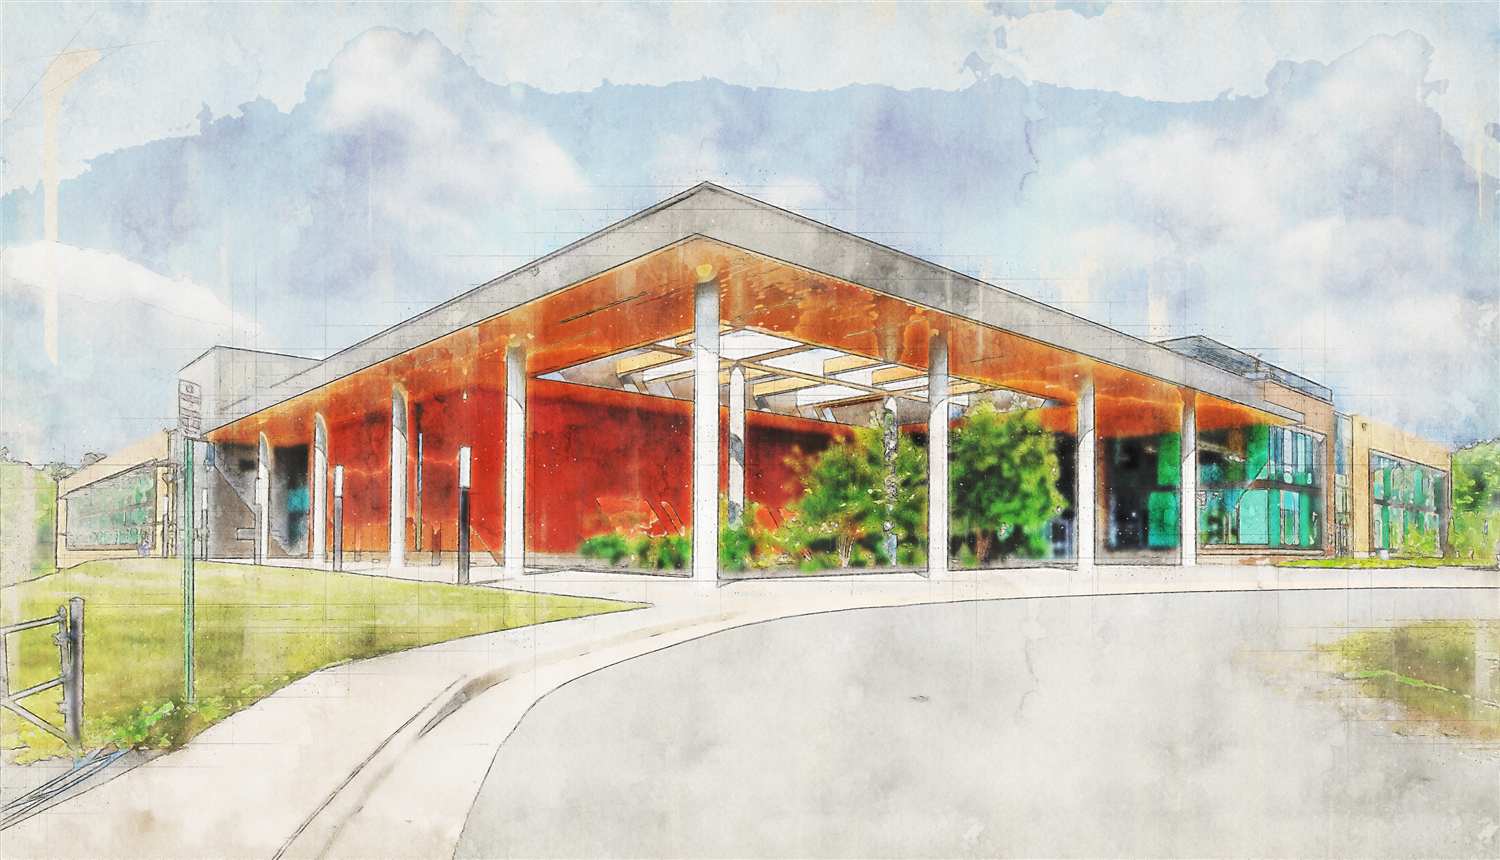
\includegraphics{./assets/acl.png}
  
  {\Huge ACL-IT 2025 Problemset}
  
  {\Large March 23, 2025}
  
  \vspace*{\stretch{2}}
\end{titlepage}

\begin{problem}
  \problemtitle{First Day}
  \problemdesc{
    First day of school! Mr. Markley has everyone introduce themselves. Help
    Ralph introduce himself by saying ``Hello I’m Ralph!'' to others around him.
  }
  \probleminput{
    You will be given a single newline-terminated string. The length of the
    string will not exceed 100 characters (including the newline).
  }
  \problemoutput{
    Print out exactly ``Hello [\emph{input}] I'm Ralph!'', terminated by a newline.
  }
  \problemsamplein{%
    Dr. Priddy
    
    Ralph
  }
  \problemsampleout{%
    Hello Dr. Priddy I'm Ralph!

    Hello Ralph I'm Ralph!
  }
  \problemexplain{Explain the sample test cases here.}
\end{problem}

\begin{problem}
  \problemtitle{Title of the Problem}
  \problemdesc{Write the description for the problem here.}
  \probleminput{Describe the input format here.}
  \problemoutput{Describe the output format here.}
  \problemsamplein{Sample input goes here.}
  \problemsampleout{Sample output goes here.}
  \problemexplain{Explain the sample test cases here.}
\end{problem}

\end{document}
